\notechapter{N-20261109}{Twenty-Seven Lines on a Cubic Surface}

A general surface of degree \(3\) in projective three-space contains exactly twenty-seven complex projective lines, provided the surface is smooth. The number has appeared in classical geometry for almost two centuries, and it looks unlikely at first sight. A plane contains far too many lines to count; a smooth quadric surface carries two entire one-parameter families of lines. Then, at degree three, the answer suddenly becomes a finite integer:
\[
 \boxed{27}.
\]

The best way I know to make that number less mysterious is to leave three-dimensional space for a while and work in the projective plane. Six points, a small geometric surgery at each of them, and some elementary intersection arithmetic will produce every one of the twenty-seven lines. The geometry is classical; the modern language is that of blow-ups and del Pezzo surfaces.\footnote{For the classical cubic-surface geometry, see Igor Dolgachev, \emph{Classical Algebraic Geometry: A Modern View} (2012), Chapters 8--9. The blow-up method and intersection-theoretic counting argument are also presented in Ravi Vakil's \href{https://math.stanford.edu/~vakil/02-245/sclass14A.pdf}{\emph{Complex Algebraic Surfaces}, Class 14}.}

\section{Why a line on a cubic is special}

Work over \(\mathbb C\). A projective line in \(\mathbb P^3\) is the set of one-dimensional linear subspaces of a fixed two-dimensional subspace of \(\mathbb C^4\). A smooth cubic surface is the zero set
\[
 S=\{[x_0:x_1:x_2:x_3]\in\mathbb P^3:
       F(x_0,x_1,x_2,x_3)=0\},
\]
where \(F\) is homogeneous of degree three and its four partial derivatives never vanish simultaneously on \(S\).

If we choose an arbitrary projective line \(\ell\subset\mathbb P^3\), the restriction \(F|_\ell\) is a homogeneous cubic in the line's two coordinates. For \(\ell\) to lie \emph{entirely} in \(S\), all four coefficients of this restricted cubic must vanish.

The space of lines in \(\mathbb P^3\), the Grassmannian \(\operatorname{Gr}(2,4)\), has dimension four. Requiring four coefficients to vanish suggests a zero-dimensional set of solutions. This is a useful dimension count, though it does not prove that the set is finite or that its cardinality is 27.

An instructive comparison is a smooth quadric:
\[
 x_0x_3-x_1x_2=0.
\]
It is the image of the Segre map
\[
 ([s_0:s_1],[t_0:t_1])
 \longmapsto
 [s_0t_0:s_0t_1:s_1t_0:s_1t_1],
\]
so the surface is isomorphic to \(\mathbb P^1\times\mathbb P^1\). Holding either factor fixed gives a whole family of lines. The cubic surface is a different creature.

\section{Replacing a point by its directions}

Take the affine plane with coordinates \((x,y)\) and blow up the origin. The construction is surprisingly explicit:
\begin{equation}
 \operatorname{Bl}_0\mathbb A^2=
 \{((x,y),[u:v])\in\mathbb A^2\times\mathbb P^1:
                         xv=yu\}.
 \label{eq:N20261109-blowup-local}
\end{equation}
There is a natural projection
\[
 \pi:\operatorname{Bl}_0\mathbb A^2\longrightarrow\mathbb A^2,
 \qquad((x,y),[u:v])\longmapsto(x,y).
\]
Away from the origin, \([u:v]=[x:y]\) is uniquely determined. Over the origin, the relation \(0=0\) imposes no condition, so
\[
 \pi^{-1}(0,0)=\{(0,0)\}\times\mathbb P^1.
\]
The single point has been replaced by an entire projective line of directions. This new curve is the \emph{exceptional divisor} \(E\).

In the chart \(u\ne0\), write \(s=v/u\). The blow-up equation becomes \(y=xs\); the exceptional divisor is \(x=0\), and \(s\) records the slope of a line approaching the origin. Thus the point where several curves met is opened into a family of directions. Curves with distinct tangent directions now meet \(E\) at distinct points.

We can carry out this operation at six distinct points \(p_1,\ldots,p_6\in\mathbb P^2\). Denote the resulting smooth surface by
\[
 \pi:S\longrightarrow\mathbb P^2.
\]
The six exceptional curves are \(E_1,\ldots,E_6\).

Choose the points in \emph{general position}: no three are collinear, and no conic passes through all six. These are the conditions that will make the anticanonical map an embedding into a smooth cubic surface.

\section{Counting using divisors}

A divisor class on \(S\) can be expressed in terms of
\[
 H=\pi^*[\text{a line in }\mathbb P^2],
 \qquad E_1,\ldots,E_6.
\]
The intersection pairing is determined by
\begin{equation}
 H^2=1,\qquad H\cdot E_i=0,\qquad
 E_i\cdot E_j=-\delta_{ij}.
 \label{eq:N20261109-intersection}
\end{equation}
The sign in \(E_i^2=-1\) may look strange. Geometrically the exceptional curve is a projective line with a negative normal bundle; intersection theory keeps track of the fact that it came from contracting a point.

The canonical divisor satisfies the blow-up formula
\[
 K_S=\pi^*K_{\mathbb P^2}+\sum_{i=1}^6E_i
     =-3H+\sum_{i=1}^6E_i.
\]
Put
\begin{equation}
 A=-K_S=3H-\sum_{i=1}^6E_i.
 \label{eq:N20261109-anticanonical}
\end{equation}
Then
\[
 A^2=9-6=3.
\]
The linear system \(|A|\) consists of plane cubic curves passing through our six points, with their proper transforms on \(S\). Plane cubics form a ten-dimensional vector space of homogeneous forms; six general point conditions reduce the dimension to four. The resulting projective linear system maps \(S\) to \(\mathbb P^3\).

A classical del Pezzo surface theorem says that, for six points in general position, the divisor \(A\) is very ample. Thus this map is an embedding. Its image has degree
\[
 \deg\varphi_A(S)=A^2=3,
\]
so it is a smooth cubic surface in \(\mathbb P^3\). We have found a way to \emph{construct} a smooth cubic surface out of six points in a plane.

Moreover, the same classical classification theorem identifies every smooth cubic surface over \(\mathbb C\) with a blow-up of six points in general position. The usual proof uses the existence and contraction of six mutually skew lines on the cubic. We take this geometric classification as an input; the numerical count below will be proved directly from the intersection pairing.

\section{Three kinds of curves}

Once the six points have been chosen, three families of curves are immediately visible.

\paragraph{The six exceptional curves.}
Each blown-up point yields \(E_i\), with
\[
 E_i^2=-1,\qquad A\cdot E_i=1.
\]
Since its degree under the anticanonical embedding is one, \(E_i\) maps to a projective line in \(\mathbb P^3\). We have six lines already.

\paragraph{The fifteen lines through pairs of points.}
For \(1\leq i<j\leq6\), the unique plane line through \(p_i\) and \(p_j\) has proper transform
\[
 L_{ij}=H-E_i-E_j.
\]
It has
\[
 L_{ij}^2=1-1-1=-1,\qquad
 A\cdot L_{ij}=3-1-1=1.
\]
Thus each \(L_{ij}\) becomes a line on the cubic surface. There are
\[
 \binom62=15
\]
of them.

\paragraph{The six conics through five points.}
For each \(i\), the other five points determine a conic. Its proper transform has class
\[
 Q_i=2H-\sum_{j\ne i}E_j.
\]
General position ensures that it is irreducible and avoids the sixth point. Again,
\[
 Q_i^2=4-5=-1,\qquad A\cdot Q_i=6-5=1.
\]
So these six conics also become projective lines under the anticanonical embedding.

We have produced
\begin{equation}
 \underbrace{6}_{E_i}
 +\underbrace{15}_{L_{ij}}
 +\underbrace{6}_{Q_i}
 =27
 \label{eq:N20261109-6-15-6}
\end{equation}
distinct lines. The surprising number now has a very simple combinatorial origin. Yet a count of 27 \emph{known} lines does not exclude the existence of a twenty-eighth. The exclusion is where intersection theory earns its keep.

\section{Why there cannot be a twenty-eighth}

Let \(C\subseteq S\) be any line in the cubic embedding, viewed as a curve on our blown-up plane. Because the embedding is given by \(A=-K_S\), its degree is
\[
 A\cdot C=1.
\]
A line is a smooth rational curve, hence has genus \(0\). The adjunction formula reads
\[
 2g(C)-2=C^2+K_S\cdot C.
\]
Substituting \(g(C)=0\) and \(K_S\cdot C=-1\) gives
\begin{equation}
 C^2=-1.
 \label{eq:N20261109-minusone}
\end{equation}

If \(C\) equals one of the exceptional curves \(E_i\), it is already on our list. Otherwise \(C\) is an irreducible curve distinct from every \(E_i\), so the intersection number \(C\cdot E_i\) is nonnegative. Write its divisor class as
\[
 C=dH-\sum_{i=1}^6m_iE_i,
 \qquad d\in\mathbb Z,\quad m_i\in\mathbb Z_{\geq0}.
\]
The coefficients have a geometric interpretation: \(d\) is the degree of the curve's image in the plane, and \(m_i\) is its multiplicity at \(p_i\). Because \(C\) is not exceptional, \(d\geq1\).

The two numerical conditions just obtained become
\begin{equation}
 3d-\sum_{i=1}^6m_i=1,
 \qquad
 d^2-\sum_{i=1}^6m_i^2=-1.
 \label{eq:N20261109-diophantine}
\end{equation}
Thus
\[
 \sum_i m_i=3d-1,\qquad
 \sum_i m_i^2=d^2+1.
\]
Apply Cauchy--Schwarz to the six integers \(m_i\):
\[
 \left(\sum_i m_i\right)^2
 \leq6\sum_i m_i^2.
\]
Substitution yields
\[
 (3d-1)^2\leq6(d^2+1),
 \qquad
 3d^2-6d-5\leq0.
\]
For an integer \(d\geq1\), this forces
\[
 \boxed{d=1\quad\text{or}\quad d=2.}
\]
That bound is the decisive step. Every possible nonexceptional line on the cubic must arise from a plane curve of degree one or two.

If \(d=1\), the equations say
\[
 \sum_i m_i=2,\qquad\sum_i m_i^2=2.
\]
Since the \(m_i\) are nonnegative integers,
\(\sum_i m_i(m_i-1)=0\), so every \(m_i\) is \(0\) or \(1\). Exactly two of them equal \(1\). This recovers the fifteen classes \(H-E_i-E_j\).

If \(d=2\), similarly,
\[
 \sum_i m_i=5,\qquad\sum_i m_i^2=5.
\]
Exactly five \(m_i\) equal \(1\), recovering the six conic classes \(2H-\sum_{j\ne i}E_j\).

No further cases exist. The possibilities are exhausted by six exceptional curves, fifteen pair-lines and six five-point conics.

\begin{theorem}[The twenty-seven lines]
Every smooth cubic surface in \(\mathbb P^3_{\mathbb C}\) contains exactly \(27\) projective lines. Under its presentation as the blow-up of \(\mathbb P^2\) at six points in general position, their classes are
\[
 \begin{aligned}
 E_i\quad&(1\leq i\leq6),\\
 H-E_i-E_j\quad&(1\leq i<j\leq6),\\
 2H-\sum_{j\ne i}E_j\quad&(1\leq i\leq6).
 \end{aligned}
\]
\end{theorem}

The proof has two logically distinct ingredients. The classical classification identifies an arbitrary smooth cubic with a six-point blow-up. Once that identification is made, the complete list and the absence of extra lines follow from the two intersection equations and one Cauchy--Schwarz inequality.

\section{The intersections are just arithmetic}

The divisor classes do more than count the lines. They tell us precisely which pairs of lines meet. Distinct irreducible curves on a smooth surface have nonnegative intersection number, and in this configuration the number is either \(0\) or \(1\). Zero means the curves are disjoint; one means they meet at a single point, counted with multiplicity.

Let the symbols \(E_i,L_{ij},Q_i\) denote the 27 lines as above. Using \eqref{eq:N20261109-intersection}, we find
\begin{align}
 E_i\cdot E_j&=0 &&(i\ne j),\notag\\
 Q_i\cdot Q_j&=0 &&(i\ne j),\notag\\
 E_i\cdot Q_j&=
 \begin{cases}0,&i=j,\\1,&i\ne j,\end{cases}\notag\\
 E_k\cdot L_{ij}&=
 \begin{cases}1,&k\in\{i,j\},\\0,&k\notin\{i,j\},\end{cases}
 \label{eq:N20261109-incidence}\\
 L_{ij}\cdot Q_k&=
 \begin{cases}1,&k\in\{i,j\},\\0,&k\notin\{i,j\},\end{cases}\notag\\
 L_{ij}\cdot L_{kl}&=
 \begin{cases}1,&\{i,j\}\cap\{k,l\}=\varnothing,\\
 0,&|\{i,j\}\cap\{k,l\}|=1,
 \end{cases}
 \quad (ij\ne kl).\notag
\end{align}

For instance, why do the two lines \(L_{12}\) and \(L_{34}\) meet? Their plane ancestors are lines through disjoint pairs of points. Two projective lines in the plane meet in one point, and that point is different from all six blow-up centers. The intersection survives the blow-up. On the other hand, \(L_{12}\) and \(L_{13}\) meet in the original plane at \(p_1\). Blowing up \(p_1\) separates their distinct tangent directions, so their proper transforms are disjoint. The algebra records this:
\[
 (H-E_1-E_2)\cdot(H-E_3-E_4)=1,\qquad
 (H-E_1-E_2)\cdot(H-E_1-E_3)=0.
\]

Choose any exceptional line \(E_i\). It meets five of the \(L_{ij}\), one for each \(j\ne i\), and five of the \(Q_j\), again for \(j\ne i\). So
\[
 \boxed{\text{every line meets exactly ten of the other 26 lines}.}
\]
The same count follows for any \(L_{ij}\) or \(Q_i\) by the formulas, or from the symmetry discussed later. The graph whose vertices are the 27 lines and whose edges mean intersection is a highly regular finite graph: it has
\[
 \frac{27\cdot10}{2}=135
\]
edges.

\section{Forty-five tritangent planes}

The intersection pattern contains another lovely number. A \emph{tritangent plane} is a plane whose intersection with the cubic surface is the union of three lines:
\[
 S\cap\Pi=L_1+L_2+L_3.
\]
Because a hyperplane section of \(S\) has class \(A=-K_S\), three line classes form a tritangent section when their sum equals \(A\).

For any two distinct indices \(i,j\),
\[
 E_i+L_{ij}+Q_j
 =E_i+(H-E_i-E_j)
       +\left(2H-\sum_{k\ne j}E_k\right)
 =3H-\sum_{k=1}^6E_k=A.
\]
These three curves meet pairwise, so they indeed form a plane section. There are \(6\cdot5=30\) choices of ordered pair \((i,j)\), giving 30 tritangent planes.

There is one more family. Partition \(\{1,2,3,4,5,6\}\) into three unordered pairs, say \(\{i,j\},\{k,l\},\{m,n\}\). Then
\[
 L_{ij}+L_{kl}+L_{mn}=A,
\]
and the three lines meet pairwise because their index pairs are disjoint. The number of partitions into three unordered pairs is
\[
 \frac{6!}{(2!)^3\,3!}=15.
\]
Together these give
\begin{equation}
 \boxed{30+15=45\text{ tritangent planes}.}
 \label{eq:N20261109-tritangent}
\end{equation}

These are all the possibilities: any tritangent plane consists of three of our 27 line classes. If one is an \(E_i\), the degree and intersection equations force the other two to have degrees \(1\) and \(2\) in the plane and to be \(L_{ij}\) and \(Q_j\). If none is exceptional, the three possible degrees are \(1\) or \(2\), and their sum must equal the coefficient \(3\) of \(H\) in \(A\); hence all three are \(L\)-type curves, giving a partition into three pairs.

\begin{figure}[htbp]
\centering
\begin{tikzpicture}[>=Stealth,thick,every node/.style={font=\small}]
 \node[draw=purple!70!black,fill=purple!5,rounded corners=3pt,
       inner sep=8pt] (e) at (-2.4,0) {\(E_i\)};
 \node[draw=teal!70!black,fill=teal!6,rounded corners=3pt,
       inner sep=8pt] (l) at (0,2) {\(L_{ij}\)};
 \node[draw=orange!80!black,fill=orange!7,rounded corners=3pt,
       inner sep=8pt] (q) at (2.4,0) {\(Q_j\)};
 \draw[purple!65!black] (e)--node[above left] {\(\cdot=1\)} (l);
 \draw[teal!65!black] (l)--node[above right] {\(\cdot=1\)} (q);
 \draw[orange!75!black] (e)--node[below] {\(\cdot=1\)} (q);
 \node[below,font=\footnotesize] at (0,-.82)
  {\(E_i+L_{ij}+Q_j=A\), for \(i\ne j\)};
\end{tikzpicture}
\caption{One of the 30 tritangent triples of mixed types. Its three lines meet pairwise and their divisor classes sum to a hyperplane section of the cubic surface.}
\label{fig:N20261109-tritangent}
\end{figure}

\section{A double-six}

Arrange the six exceptional lines and the six conic lines in two rows:
\[
 \begin{pmatrix}
 E_1&E_2&E_3&E_4&E_5&E_6\\
 Q_1&Q_2&Q_3&Q_4&Q_5&Q_6
 \end{pmatrix}.
\]
The lines within either row are mutually disjoint. Across the rows, \(E_i\) meets \(Q_j\) precisely when \(i\ne j\); corresponding entries \(E_i,Q_i\) are disjoint. This arrangement is known as a \emph{Schl\"afli double-six}.

It is quite a rigid object. Given one row of six mutually skew lines on a cubic surface, the complementary row in a double-six is determined. One can contract the first six lines to obtain a projective plane, and the second row then appears as the six conics through five of the contracted points.

There are \(36\) different double-sixes among the 27 lines. That number is a classical fact about the configuration, and it can be computed from its full symmetry group. One striking consequence is that the six-point blow-up presentation is far from unique: a single cubic surface admits many different choices of six skew lines to contract to a plane.

\section{Why an \(E_6\) root system appears}

The intersection form on divisor classes has signature \((1,6)\):
\[
 \operatorname{Pic}(S)\cong\mathbb ZH
 \oplus\bigoplus_{i=1}^6\mathbb ZE_i,
 \qquad
 (H^2,E_1^2,\ldots,E_6^2)=(1,-1,\ldots,-1).
\]
The canonical divisor \(K_S=-3H+\sum_iE_i\) satisfies \(K_S^2=3>0\). Its orthogonal complement
\[
 K_S^\perp=\{D\in\operatorname{Pic}(S):D\cdot K_S=0\}
\]
has rank six and a negative-definite intersection pairing.

Consider six particularly simple classes:
\begin{equation}
 \alpha_i=E_i-E_{i+1}\quad(1\leq i\leq5),
 \qquad
 \alpha_6=H-E_1-E_2-E_3.
 \label{eq:N20261109-simple-roots}
\end{equation}
Direct calculation using \eqref{eq:N20261109-intersection} gives
\[
 K_S\cdot\alpha_i=0,\qquad \alpha_i^2=-2,
\]
and
\[
 \alpha_i\cdot\alpha_j=
 \begin{cases}
 1,&\text{\(i,j\) adjacent in the diagram below},\\
 0,&i\ne j\text{ and not adjacent}.
 \end{cases}
\]
The diagram is the Dynkin diagram of the exceptional root system \(E_6\).

\begin{figure}[htbp]
\centering
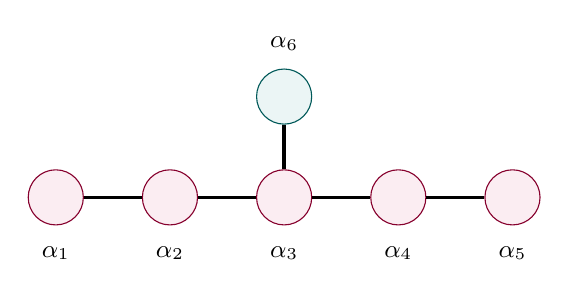
\begin{tikzpicture}[every node/.style={font=\small}]
 \foreach \i/\x in {1/0,2/1.45,3/2.90,4/4.35,5/5.80}{
  \node[draw=purple!70!black,fill=purple!7,circle,
    minimum size=7mm] (a\i) at (\x,0) {};
  \node[below=4pt] at (a\i.south) {\(\alpha_{\i}\)};
 }
 \node[draw=teal!70!black,fill=teal!8,circle,
   minimum size=7mm] (a6) at (2.90,1.28) {};
 \node[above=3pt] at (a6.north) {\(\alpha_6\)};
 \draw[very thick] (a1)--(a2)--(a3)--(a4)--(a5);
 \draw[very thick] (a3)--(a6);
\end{tikzpicture}
\caption{The six roots extracted from the intersection pairing form an \(E_6\) Dynkin diagram. Adjacency means intersection number \(1\), and every root has self-intersection \(-2\).}
\label{fig:N20261109-E6}
\end{figure}

To turn these classes into symmetries, use the reflection associated to a root \(\alpha\) with \(\alpha^2=-2\):
\begin{equation}
 s_\alpha(D)=D+(D\cdot\alpha)\alpha.
 \label{eq:N20261109-reflection}
\end{equation}
It fixes every class orthogonal to \(\alpha\), sends \(\alpha\) to \(-\alpha\), and preserves the intersection pairing. Since \(K_S\cdot\alpha=0\), it also fixes the canonical class. Thus the reflection preserves the two numerical conditions
\[
 D^2=-1,\qquad (-K_S)\cdot D=1.
\]
Our classification says that these conditions, together with the appropriate effective line classes, produce exactly the 27 possibilities. Indeed these root reflections permute that finite set.

One calculation makes the symmetry surprisingly concrete. For
\(\alpha_6=H-E_1-E_2-E_3\), we have \(E_1\cdot\alpha_6=1\), and hence
\begin{align*}
 s_{\alpha_6}(E_1)
 &=E_1+(E_1\cdot\alpha_6)\alpha_6\\
 &=H-E_2-E_3\\
 &=L_{23}.
\end{align*}
A reflection in the root lattice exchanges the class of an exceptional curve with the class of a line through two of the blown-up points! It can mix the three families that gave the count \(6+15+6\).

The group generated by the reflections in the \(E_6\) roots is the Weyl group \(W(E_6)\). A classical theorem identifies it with the full automorphism group of the intersection graph of the 27 lines. Its order is
\begin{equation}
 |W(E_6)|=2\cdot5\cdot6\cdot8\cdot9\cdot12
 =51840.
 \label{eq:N20261109-WeylOrder}
\end{equation}
The factors are the degrees of the basic polynomial invariants of the \(E_6\) reflection representation. Establishing the invariant-theoretic result is beyond the counting proof; here the visible geometric content is the explicit root lattice, its reflection formula and its action on the line classes.

It is important to identify which symmetry we are speaking about. The Weyl group describes the \emph{incidence configuration} of the 27 lines, not necessarily the group of projective automorphisms of one fixed cubic surface. A general smooth cubic has no nontrivial projective automorphisms, even though its 27 lines have the entire abstract \(W(E_6)\) incidence symmetry.

\section{Twenty-seven lines in one explicit equation}

After all this intersection theory, it is pleasant to return to an equation one can check by substitution. Consider the Fermat cubic
\begin{equation}
 S_F:\quad x_0^3+x_1^3+x_2^3+x_3^3=0
 \qquad\text{in }\mathbb P^3_{\mathbb C}.
 \label{eq:N20261109-fermat}
\end{equation}
It is smooth: the four partial derivatives are \(3x_i^2\), and they cannot all vanish at a projective point.

Divide the four indices into two unordered pairs, for example
\(\{0,1\}\sqcup\{2,3\}\). For any two cube roots of unity
\(\zeta^3=\eta^3=1\), impose the linear equations
\begin{equation}
 x_0+\zeta x_1=0,\qquad x_2+\eta x_3=0.
 \label{eq:N20261109-fermat-lines}
\end{equation}
They define a projective line. On that line,
\[
 x_0^3+x_1^3=(-\zeta)^3x_1^3+x_1^3=0,
\]
and likewise \(x_2^3+x_3^3=0\), so the line lies entirely on \(S_F\).

There are three ways to partition four indices into two pairs:
\[
 \begin{gathered}
 \{0,1\}\sqcup\{2,3\},\\
 \{0,2\}\sqcup\{1,3\},\\
 \{0,3\}\sqcup\{1,2\}.
 \end{gathered}
\]
For each partition there are three choices of \(\zeta\) and three of \(\eta\), yielding nine lines. The choices give distinct projective lines, hence
\begin{equation}
 \underbrace{3}_{\text{pairings}}\times
 \underbrace{3}_{\zeta}\times
 \underbrace{3}_{\eta}
 =27
 \label{eq:N20261109-fermat-count}
\end{equation}
explicit lines on the smooth Fermat cubic. Our classification theorem says these are \emph{all} of them.

This short calculation provides a complementary view of the famous number. In the blow-up picture, \(27\) arose as \(6+15+6\); in one particularly symmetric equation it appears as \(3\cdot3\cdot3\). The two enumerations concern the same geometric objects, although their indexing systems look completely different.

There is a small extra twist if we insist on \emph{real} lines. The equation \eqref{eq:N20261109-fermat} has real coefficients, but most of its 27 complex lines do not lie in real projective space. Complex conjugation sends the line specified by \((\zeta,\eta)\) to the line specified by \((\overline\zeta,\overline\eta)\). For a fixed pairing, the three cube roots of unity are
\[
 1,\qquad\omega=e^{2\pi i/3},\qquad
 \omega^2=\overline\omega.
\]
Only \(1\) is real. Since all the lines in our explicit list are distinct, a line is fixed by conjugation precisely when both parameters equal \(1\). There is exactly one such line for each of the three pairings, so
\[
 \boxed{\#\{\text{real lines on }S_F\}=3.}
\]
Thus the same smooth cubic surface that has 27 lines over \(\mathbb C\) has just three lines defined over \(\mathbb R\).

The parity is no accident. For \emph{any} smooth cubic surface defined by a real equation, complex conjugation permutes its 27 complex lines. Every orbit has one or two elements; a line fixed by conjugation is a real line, while a nonreal line belongs to a two-element conjugate pair. Because 27 is odd, the number of real lines must also be odd. This easy argument does not determine the number, but it extracts a genuine arithmetic constraint from a purely geometric count.

\section{Following twenty-seven lines around a loop}

There is one last connection to the geometry of polynomial roots. In our earlier note on monodromy, the roots of \(z^3-3z=t\) were continued along paths in the parameter plane. Two simple branch points produced transpositions and, together, the group \(S_3\).

For cubic surfaces the \emph{coefficients of the cubic equation} can also move. Why should its 27 lines then admit locally continuous labels, as the roots of a polynomial do? The self-intersection calculation provides the local rigidity needed for an answer.

A line \(L\subset S\) is a smooth rational curve, so \(L\cong\mathbb P^1\). Its normal bundle inside the surface is a line bundle whose degree is \(L^2=-1\):
\[
 N_{L/S}\cong\mathcal O_{\mathbb P^1}(-1).
\]
Infinitesimal deformations of \(L\) \emph{within a fixed surface} are parametrized by \(H^0(L,N_{L/S})\). Since
\[
 H^0(\mathbb P^1,\mathcal O(-1))=0,
\]
there is no nontrivial first-order deformation of a line while the surface remains fixed. This is the infinitesimal reason the lines form a discrete set.

The corresponding obstruction space is \(H^1(L,N_{L/S})\), which also vanishes for \(\mathcal O(-1)\). Standard deformation theory therefore says that when we vary the smooth cubic surface slightly, each of its lines moves uniquely and smoothly with that variation. Equivalently, the universal family of pairs
\[
 \{(S,L): S\text{ a smooth cubic surface},\quad L\subset S
       \text{ a line}\}
\]
is locally a 27-sheeted covering over the space of smooth cubic equations (with scalar multiples identified). This is a geometric version of the implicit-function theorem for the roots of a polynomial.

A closed path through this parameter space may consequently return to the original cubic while permuting its 27 lines. We obtain a monodromy action on a set of 27 objects, just as we previously did for three polynomial roots.

For the universal family of smooth cubic surfaces, the monodromy group of the 27 lines is the full Weyl group \(W(E_6)\). This classical result can be understood from the blow-up presentations and their Cremona transformations. The relevant paths are paths \emph{in the space of cubic surfaces}; a closed path on a single fixed cubic surface is a different object.

The numerical count and the symmetry group thus come from the same elementary-looking starting data: six points in a plane. The six points give 27 line classes, the intersection pairing gives their incidences, and the classes orthogonal to the canonical divisor produce the \(E_6\) root system. A question about twenty-seven very concrete straight lines has led, through a precise chain of calculations, to one of the exceptional Weyl groups.
